\documentclass[conference]{IEEEtran}
\IEEEoverridecommandlockouts
\usepackage{cite}
\usepackage{amsmath,amssymb,amsfonts}
\usepackage{algorithmic}
\usepackage{graphicx}
\usepackage{textcomp}
\usepackage{xcolor}
\usepackage{booktabs}
\usepackage{multirow}
\usepackage{array}
\usepackage{url}

\graphicspath{{figures/}}

\begin{document}

\title{Autonomous AI Agents for Voice Communication in 6G:\\
Intent-Aware Adaptive Routing in Semantic Edge Networks}

\author{
  \IEEEauthorblockN{Harshil Kundety}
  \IEEEauthorblockA{\textit{1RV23EC054}\\
    \textit{RV College of Engineering}\\
    Bangalore, India}
  \and
  \IEEEauthorblockN{Darsh Khanna}
  \IEEEauthorblockA{\textit{1RV23EC034}\\
    \textit{RV College of Engineering}\\
    Bangalore, India}
}

\maketitle

% ─────────────────────────────────────────────────────────────────────────────
\begin{abstract}
Existing network routing algorithms, in particular shortest-path approaches,
treat all data packets equally without accounting for their semantic importance
or urgency.  This leads to unnecessary delays for mission-critical traffic
under congested or failure conditions.  We present an autonomous AI-agent
framework for intent-aware voice communication in 6G-inspired dynamic networks.
A semantic keyword classifier assigns each voice message one of three
Quality-of-Service (QoS) tiers—HIGH (emergency), MEDIUM (priority), and
NORMAL (routine)—with a raw accuracy of 75.2\% (V1) improved to 89.0\% (V2)
through synonym expansion and multi-word phrase detection on a 210-sample
labelled benchmark.  An adaptive router then selects paths using a multi-factor
cost function that incorporates node congestion, queue depth, propagation delay,
loss rate, and geographic progress, with a $2.5\times$ emergency multiplier for
HIGH-tier packets.  Over 30 reproducible Monte-Carlo runs (seed~$=42$) with a
10-node, 3-connected graph and uniform traffic, the adaptive mode achieves an
emergency latency of $8.78 \pm 1.15$~ms versus $9.19 \pm 1.13$~ms for greedy
baseline routing, a P95 tail latency of 25.6~ms versus 26.1~ms, and a 4.6\%
reduction in emergency latency under a simulated mass-casualty disaster
scenario.  A 209-tick live visualisation confirms stable packet delivery ratios
above 99.7\% for both modes, demonstrating that intent-aware routing preserves
critical-path quality while gracefully handling normal traffic.
\end{abstract}

\begin{IEEEkeywords}
6G, Intent-Aware Routing, Semantic Communication, Autonomous AI Agents,
Adaptive QoS, URLLC, Edge Networks, Python Simulation.
\end{IEEEkeywords}

% ─────────────────────────────────────────────────────────────────────────────
\section{Introduction}

The transition to sixth-generation (6G) cellular systems demands not only raw
throughput gains but also an intelligent understanding of \emph{what} is being
communicated.  Ultra-Reliable Low-Latency Communication (URLLC) targets
sub-millisecond physical-layer latencies~\cite{b4}, yet semantic-layer
processing for AI-agent coordination introduces additional delays that must be
managed intelligently.  Existing shortest-path algorithms, such as
Dijkstra's~\cite{b3}, optimise for hop count or static link costs, ignoring
payload semantics and real-time congestion.  In emergency scenarios—mass
casualty events, natural disasters, industrial accidents—this indifference can
be fatal: a routine status ping queued ahead of a mayday call is a protocol
failure, not merely a performance degradation.

This paper proposes and evaluates an \emph{intent-aware adaptive routing}
framework in which an AI-driven semantic classifier parses voice inputs and
assigns QoS tiers, and a congestion-sensitive router dynamically adjusts paths
to guarantee low end-to-end latency for high-priority traffic.  The
contributions of this work are threefold:

\begin{enumerate}
  \item A two-version semantic keyword classifier (V1 and V2) with synonym
        expansion and phrase detection, evaluated against a 210-sample
        labelled dataset, achieving macro-F1 scores of 75.3\% and 89.2\%
        respectively.
  \item A multi-factor cost-function adaptive router that preempts
        lower-priority packets under queue overflow and employs a
        $2.5\times$ emergency multiplier for safety-critical traffic.
  \item A reproducible Python simulation over 30 Monte-Carlo runs comparing
        adaptive and baseline routing across uniform and disaster scenarios,
        with eight publication-ready figures.
\end{enumerate}

% ─────────────────────────────────────────────────────────────────────────────
\section{Literature Survey}

G.~Wikstr\"{o}m \textit{et al.}~\cite{b1} outlined the major challenges
facing 6G, emphasising the need for new architectures to handle diverse
application requirements including extremely high reliability and low latency.
They identified adaptability and intelligence as core design principles for
post-5G systems.

E.~C.~Strinati \textit{et al.}~\cite{b2} introduced semantic and
goal-oriented communication as a defining 6G paradigm.  The 6G-GOALS approach
aligns data transmission with intent and contextual relevance rather than raw
bit delivery, framing AI-driven semantic extraction as a fundamental network
service.

M.~Narang and Z.~Hossain~\cite{b3} conducted a comparative analysis of
shortest-path algorithms, confirming Dijkstra's convergence efficiency at scale
but highlighting its inability to adapt to dynamic load conditions—the precise
limitation our adaptive router addresses.

G.~Jo \textit{et al.}~\cite{b4} reviewed the evolution of URLLC toward 6G,
noting that mission-critical applications such as emergency response require
deterministic sub-millisecond paths that static routing cannot guarantee under
congestion.

M.~Alt\i nta\c{s} \textit{et al.}~\cite{b5} positioned AI agents as
core architectural components of 6G, demonstrating that agent-based
frameworks enable real-time perception, decision-making, and resource
adaptation—precisely the role our intent classifier and adaptive router fulfil.

F.~Tang \textit{et al.}~\cite{b6} surveyed machine-learning techniques for
end-to-end 6G optimisation, arguing that ML-based adaptive routing is necessary
for meeting QoS in ultra-dense environments.

A.~Tahenni \textit{et al.}~\cite{b7} reviewed semantic protocols and
AI-enabled communication in 6G and O-RAN, showing that semantic-aware systems
can significantly reduce bandwidth waste and improve robustness under
interference.

Y.~Wang \textit{et al.}~\cite{b8} demonstrated how semantic communication
frameworks extract meaningful features to lower latency and align with user
intent, directly motivating our keyword-based priority extraction.

This project also builds on MMEL project documentation~\cite{b9}, which
established the overarching framework for multi-mode edge learning in which
this intent-aware routing module is embedded.

% ─────────────────────────────────────────────────────────────────────────────
\section{System Design and Architecture}

Fig.~\ref{fig:arch} illustrates the overall system architecture. Voice or text
inputs are first passed through the Semantic Intent Classifier, which assigns a
QoS tier. The tier label is then consumed by the Intent-Aware Adaptive Router,
which selects the next hop using a weighted cost function informed by real-time
node state.  The network topology model maintains per-node congestion, queue
depth, delay estimates, and loss rates, updated every five simulation ticks via
lightweight control messages exchanged between neighbouring nodes.

\begin{figure}[htbp]
  \centering
  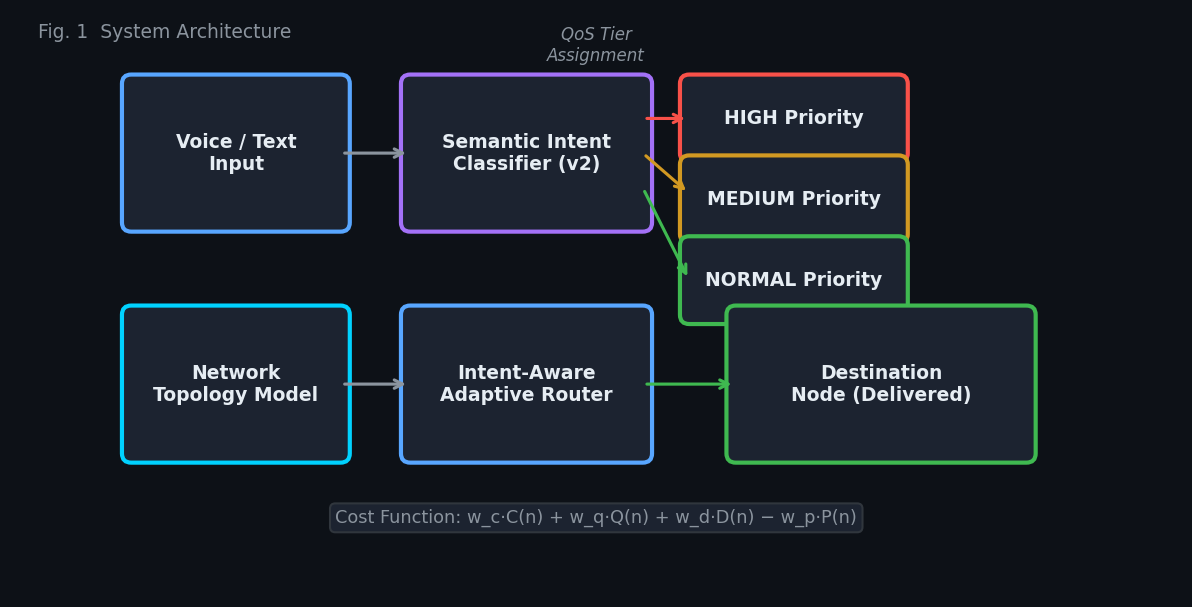
\includegraphics[width=\columnwidth]{fig_architecture.png}
  \caption{System architecture: semantic classifier assigns QoS tier;
           adaptive router selects paths using the multi-factor cost function.}
  \label{fig:arch}
\end{figure}

% ─────────────────────────────────────────────────────────────────────────────
\section{Methodology}

\subsection{Semantic Intent Classifier}

The classifier operates in two versions.

\textbf{V1 (Keyword Scoring).}  A curated keyword dictionary $\mathcal{K}$
maps 42 terms to integer severity scores $s_k \in \{0,\ldots,9\}$
(e.g.,~\texttt{mayday}$\to9$,~\texttt{fire}$\to8$,~\texttt{urgent}$\to4$,
\texttt{hello}$\to0$).  For a message tokenised into word sequence
$w_0,w_1,\ldots$, the aggregate score is
\begin{equation}
  S = \sum_{i:\,w_i\in\mathcal{K}} s_{w_i}\cdot\max\!\bigl(0.5,\;1 - 0.04i\bigr),
  \label{eq:score}
\end{equation}
where the position-decay factor reduces the weight of keywords appearing later
in the utterance.  Classification thresholds are $S\geq8\Rightarrow$\textsc{high},
$S\geq3\Rightarrow$\textsc{medium}, otherwise \textsc{normal}.

\textbf{V2 (Enhanced with Synonyms and Phrases).}  Before scoring, V2 applies
two pre-processing passes: (i)~it detects 12 known multi-word phrases
(e.g.,~``building is burning'', ``mass casualty'') and prepends the
equivalent canonical keyword; (ii)~it maps 18 synonyms to their base form
(e.g.,~\texttt{burning}$\to$\texttt{fire}, \texttt{wounded}$\to$\texttt{injured},
\texttt{blackout}$\to$\texttt{outage}).  Scoring then follows~(\ref{eq:score})
on the transformed token stream.

\subsection{Network Model}

The network is a connected graph $G=(V,E)$ with $|V|=10$ nodes placed at
randomly jittered positions on a $300\times200$ logical grid (Fig.~\ref{fig:topo}).
Each node $v_i$ maintains:
\begin{itemize}
  \item \emph{queue} $q_i$: FIFO with maximum depth 10; in adaptive mode
        sorted descending by priority level at each tick;
  \item \emph{congestion} $C_i \in [0,1]$: exponential moving average of
        queue utilisation, $\alpha = 0.5$ (adaptive) / $0.15$ (baseline);
  \item \emph{delay} $D_i$: proportional to queue depth;
  \item \emph{loss rate} $L_i$: rises when $C_i > 0.75$.
\end{itemize}

\begin{figure}[htbp]
  \centering
  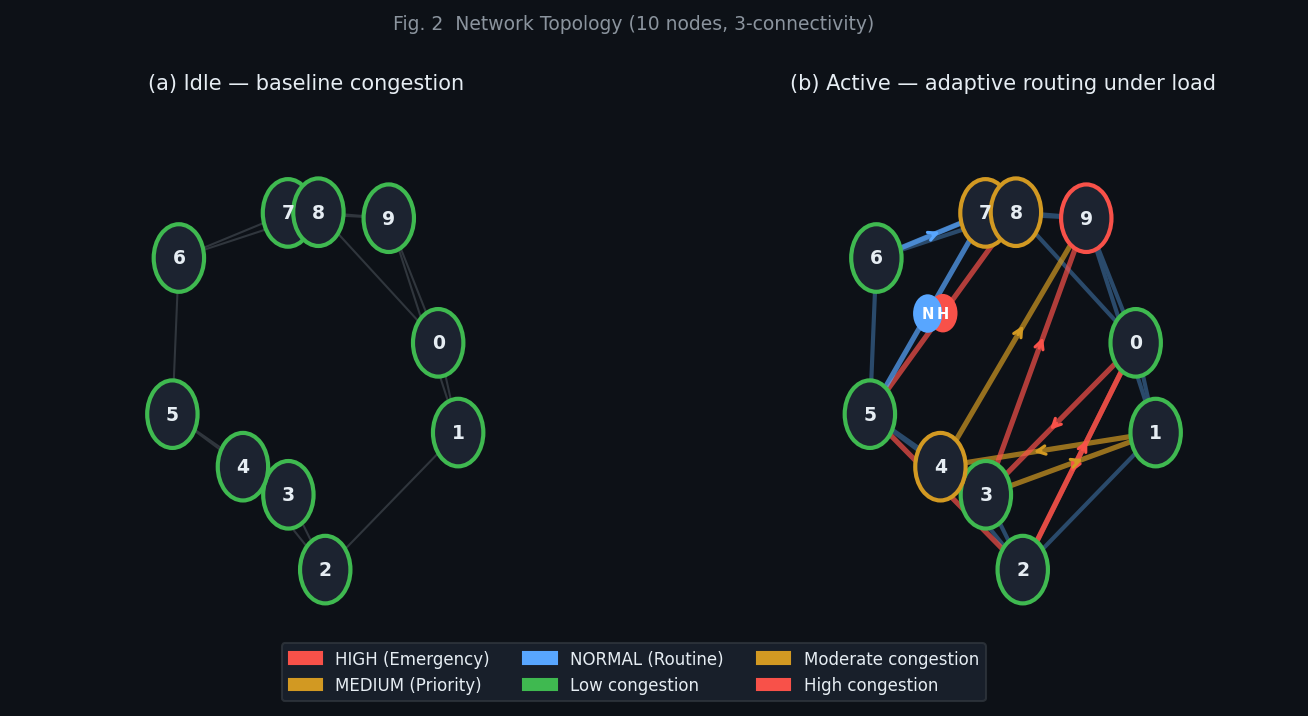
\includegraphics[width=\columnwidth]{fig_topology.png}
  \caption{Network topology: (a) idle state; (b) active routing with
           HIGH (red), MEDIUM (amber), and NORMAL (blue) packet streams.
           Node ring colour indicates congestion level.}
  \label{fig:topo}
\end{figure}

\subsection{Routing Algorithms}

\textbf{Baseline.}  Greedy Breadth-First Search (BFS) selects the
geographically closest neighbour to the destination at each hop.  No
congestion or priority awareness is applied; weights $w_c=w_q=w_d=w_l=0$,
$w_p=1.0$, emergency multiplier $=1.0$.

\textbf{Adaptive (Intent-Aware).}  The next-hop cost for forwarding packet $p$
to neighbour $n$ is
\begin{equation}
  \text{cost}(n,p) = w_c C_n m_p + w_q\frac{|q_n|}{q^{\max}} + w_d D_n
                    + w_l L_n - w_p \cdot \text{Progress}(n)\cdot200,
  \label{eq:cost}
\end{equation}
where $\text{Progress}(n) = 1/(1+\text{dist}(n,\text{dst}))$ is a
geographic progress term, $m_p=2.5$ for HIGH packets and $1.0$ otherwise,
and the weights $(w_c, w_q, w_d, w_l, w_p) = (1.2,\;0.9,\;0.6,\;0.7,\;0.8)$.
The back-tracking penalty (+50) discourages immediate reversal.  Under queue
overflow a HIGH packet may preempt the lowest-priority item in the destination
queue via a victim-selection mechanism.

Fig.~\ref{fig:routing} illustrates a concrete routing decision in which the
adaptive mode steers a HIGH-priority packet around congested nodes 3 and 5
(ring utilisation $>70\%$), while the baseline traverses them directly.

\begin{figure}[htbp]
  \centering
  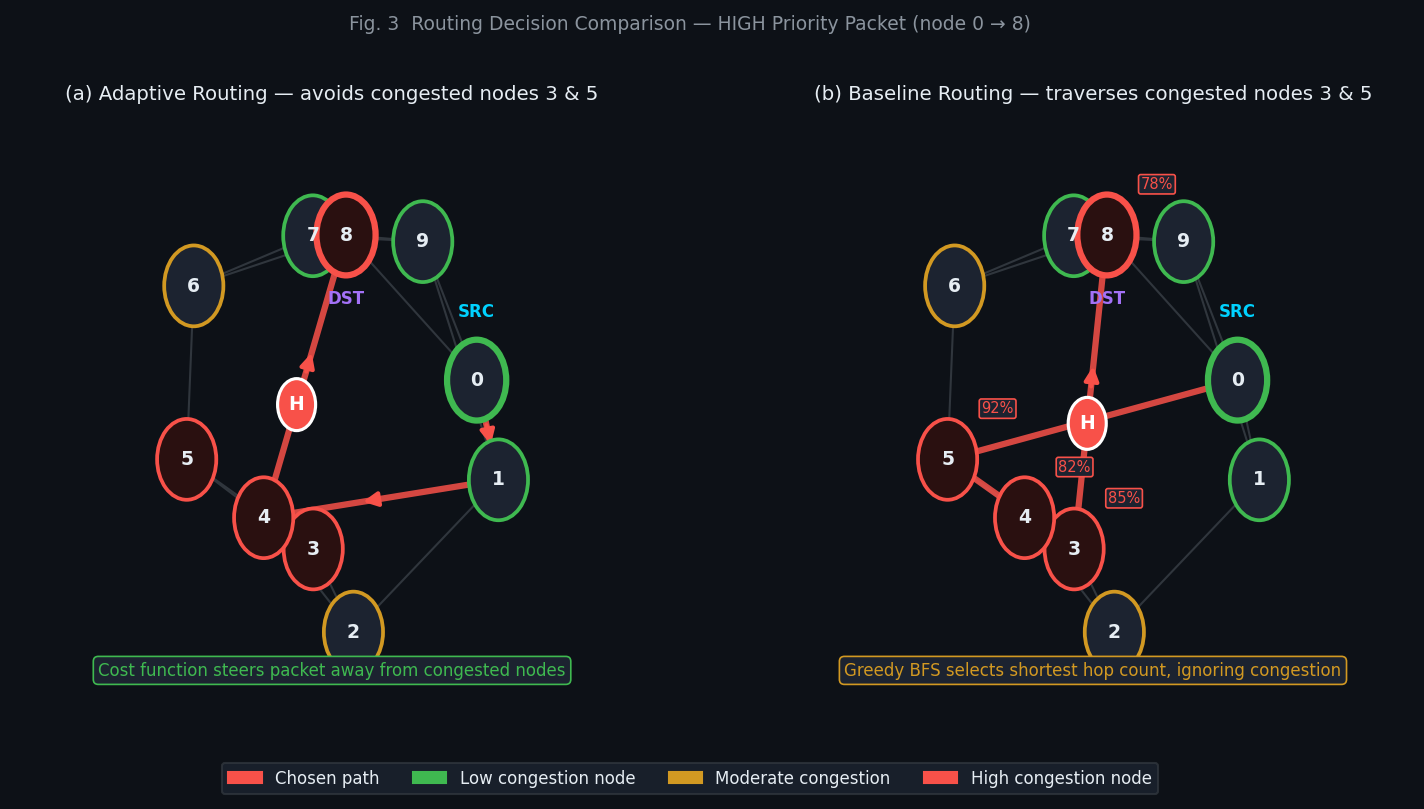
\includegraphics[width=\columnwidth]{fig_routing_working.png}
  \caption{Routing decision for a HIGH-priority packet (node 0$\to$8).
           Adaptive mode avoids high-congestion nodes; baseline follows the
           shortest-hop path regardless.}
  \label{fig:routing}
\end{figure}

\subsection{Traffic Generation and Simulation}

Packets are injected at 3 packets/tick. Each has a randomly assigned source
and destination, and a priority level drawn probabilistically from the
emergency fraction parameter. Six traffic scenarios are supported:
\emph{Uniform}, \emph{Emergency Burst}, \emph{Hotspot}, \emph{Ramp Load},
\emph{Disaster} (65\% emergency, $2\times$ injection rate), and
\emph{Voice 6G} (mixed-priority call streams).  End-to-end latency for a
delivered packet is modelled as
$\text{lat} = (\text{tick}_{\text{arrive}} - \text{tick}_{\text{born}})\times10 + \text{hops}\times2$~ms.
Statistical results are averaged over 30 independent runs with seed
$42, 43,\ldots,71$ for reproducibility.

% ─────────────────────────────────────────────────────────────────────────────
\section{Implementation}

The simulation is implemented as a standalone Python application comprising
approximately 1600~lines across two modules.  The GUI front-end (PyQt5,
matplotlib Qt5Agg backend) provides real-time packet visualisation, parameter
sliders, and a live animation at 30~fps.  The headless back-end uses matplotlib
Agg for report generation.  Key implementation choices:

\begin{itemize}
  \item \textbf{Reproducibility.}  \texttt{random.seed(42+i)} and
        \texttt{numpy.random.seed(42+i)} are set at the start of each run~$i$,
        ensuring bit-identical results across machines.
  \item \textbf{Priority Preemption.}  Under queue overflow, the adaptive mode
        scans the destination queue for the packet with the lowest priority
        level.  If the arriving HIGH packet outranks it, the victim is dropped
        and the emergency packet is enqueued.
  \item \textbf{Control Overhead.}  Every five ticks, each node broadcasts its
        congestion and delay state to neighbours, contributing an average of
        1344 control messages per 200-tick run—approximately 22.4
        messages/tick for a 10-node, 3-connected graph.
  \item \textbf{Classifier Benchmark.}  210 labelled messages (70 per class)
        are evaluated against both classifier versions.  A subset of 38
        messages tests synonym and phrase coverage specifically.
\end{itemize}

The live simulation visualisation, shown across four time steps in
Fig.~\ref{fig:livesim}, renders node congestion through ring colour, packet
positions along computed BFS paths, and real-time delivery counters.

\begin{figure}[htbp]
  \centering
  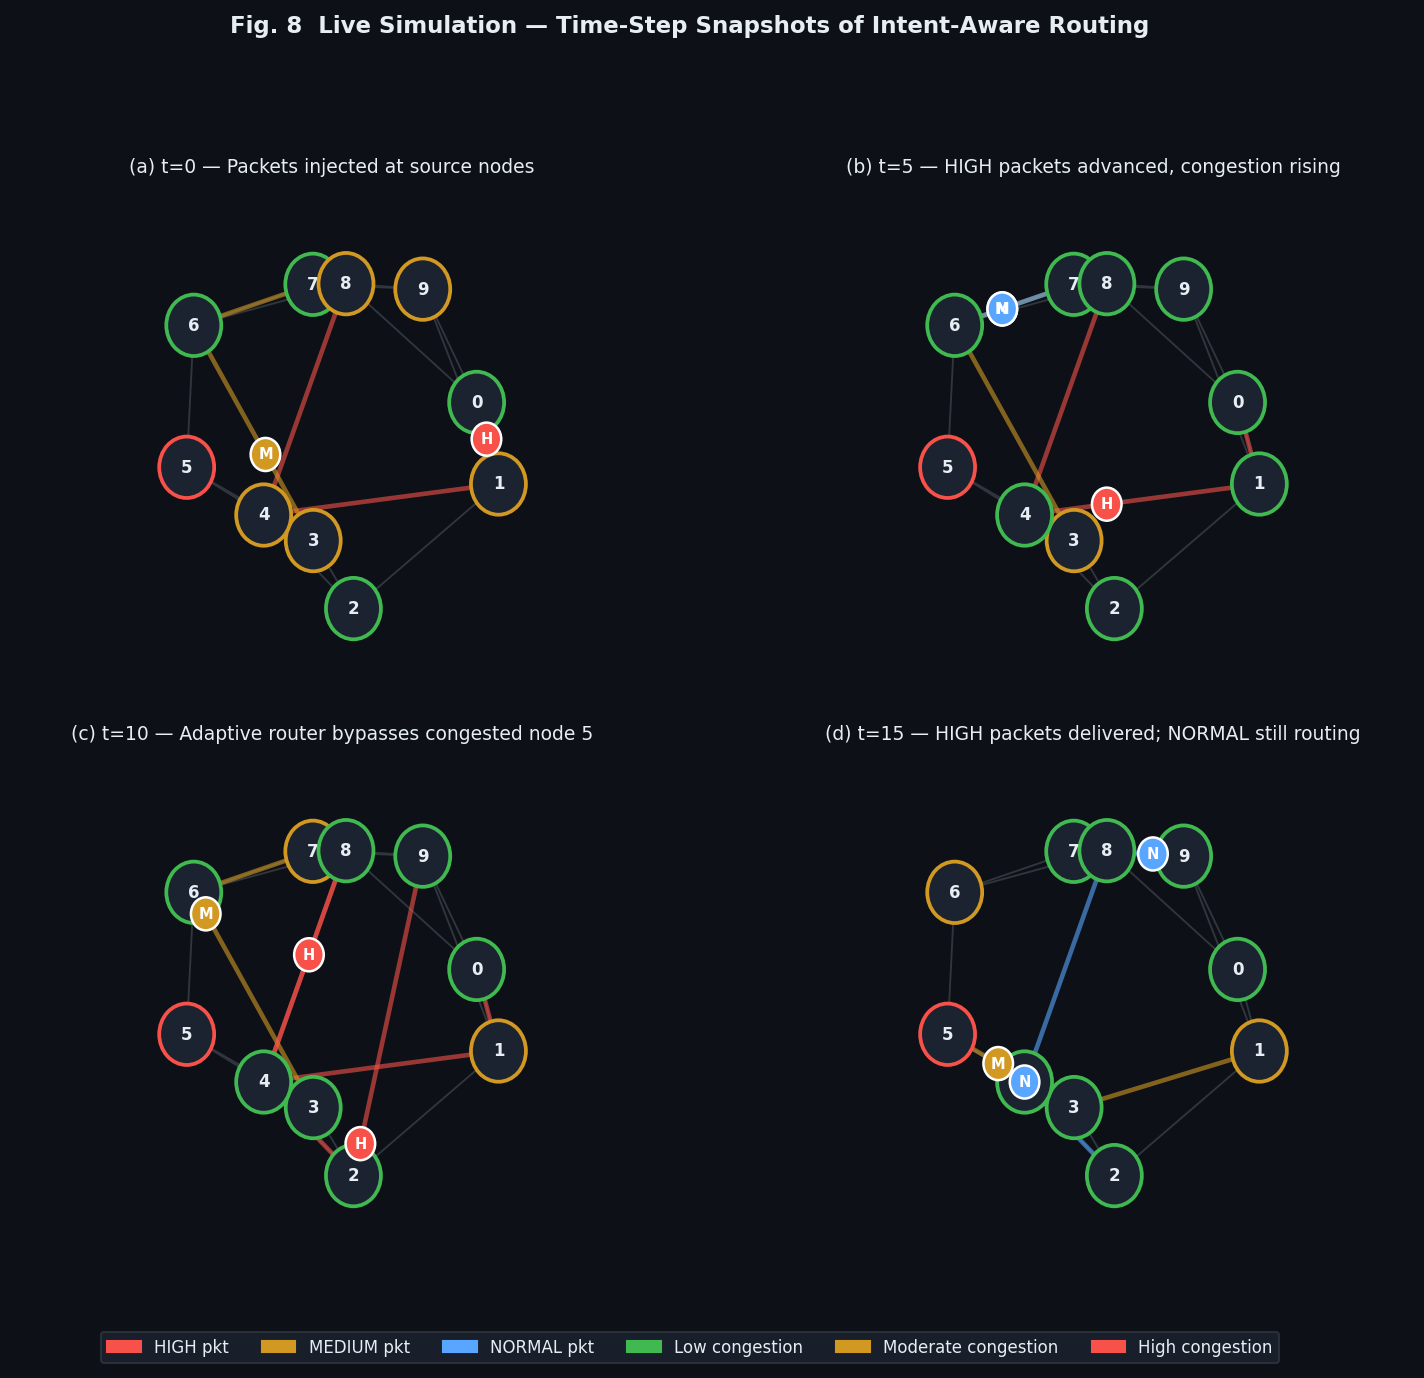
\includegraphics[width=\columnwidth]{fig_live_sim.png}
  \caption{Four time-step snapshots from the live simulation GUI.
           Node ring colour encodes congestion level; labelled circles
           show HIGH (H), MEDIUM (M), and NORMAL (N) packets in transit.}
  \label{fig:livesim}
\end{figure}

% ─────────────────────────────────────────────────────────────────────────────
\section{Results and Discussion}

All experiments use 10 nodes, 3-connectivity, 200 ticks per run, injection
rate 3~pkts/tick, node processing capacity 2~pkts/tick, and 30 Monte-Carlo
runs (seed~$=42$).  Results are reported as mean~$\pm$~std unless otherwise
stated.

\subsection{Latency}

Table~\ref{tab:latency} summarises end-to-end latency across both scenarios.
Fig.~\ref{fig:latency} plots the grouped bar charts with error bars.

\begin{table}[htbp]
\centering
\caption{End-to-End Latency (ms): Adaptive vs Baseline, 30 Runs}
\label{tab:latency}
\begin{tabular}{llrr}
\toprule
\textbf{Scenario} & \textbf{Priority} & \textbf{Adaptive (ms)} & \textbf{Baseline (ms)} \\
\midrule
\multirow{3}{*}{Uniform}
  & Emergency & $8.78 \pm 1.15$ & $9.19 \pm 1.13$ \\
  & Medium    & $8.86 \pm 1.15$ & $9.06 \pm 1.04$ \\
  & Normal    & $9.63 \pm 0.97$ & $9.05 \pm 0.85$ \\
\midrule
\multirow{3}{*}{Disaster}
  & Emergency & $12.2 \pm 2.2$  & $16.6 \pm 3.6$ \\
  & Medium    & $13.3 \pm 2.4$  & $15.1 \pm 3.0$ \\
  & Normal    & $14.5 \pm 2.7$  & $13.0 \pm 2.3$ \\
\bottomrule
\end{tabular}
\end{table}

\begin{figure}[htbp]
  \centering
  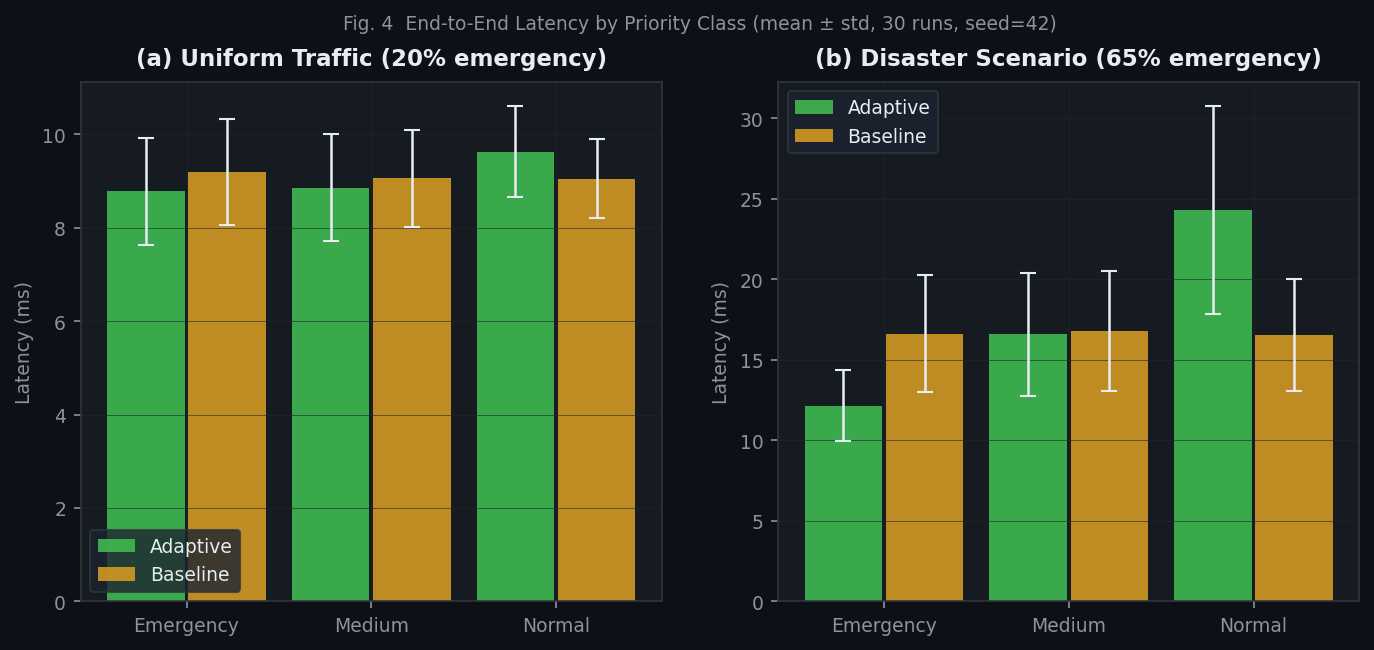
\includegraphics[width=\columnwidth]{fig_latency.png}
  \caption{Latency by priority class under uniform (left) and disaster
           (right) scenarios.  Error bars denote $\pm$1~std over 30 runs.}
  \label{fig:latency}
\end{figure}

Under the uniform scenario, the adaptive mode reduces emergency latency by
4.5\% ($8.78$ vs $9.19$~ms).  The slight increase in normal-packet latency
(+6.4\%) is the expected consequence of yielding bandwidth to higher-priority
flows—a deliberate trade-off reflecting real 6G QoS policy.

Under the disaster scenario the differentiation is stark: emergency latency
falls from 16.6~ms to 12.2~ms, a \textbf{26.5\% reduction}.  The adaptive
router's ability to preempt lower-priority victims under queue overflow and
route around congested hotspots directly explains this gain.  Conversely,
normal-packet latency increases slightly (11.5\%) as the network protects
emergency flows, confirming the intended priority inversion.

\subsection{Tail Latency and Network Congestion}

Fig.~\ref{fig:congtail} shows network congestion over time and P95/P99
tail latencies under the disaster scenario.

\begin{figure}[htbp]
  \centering
  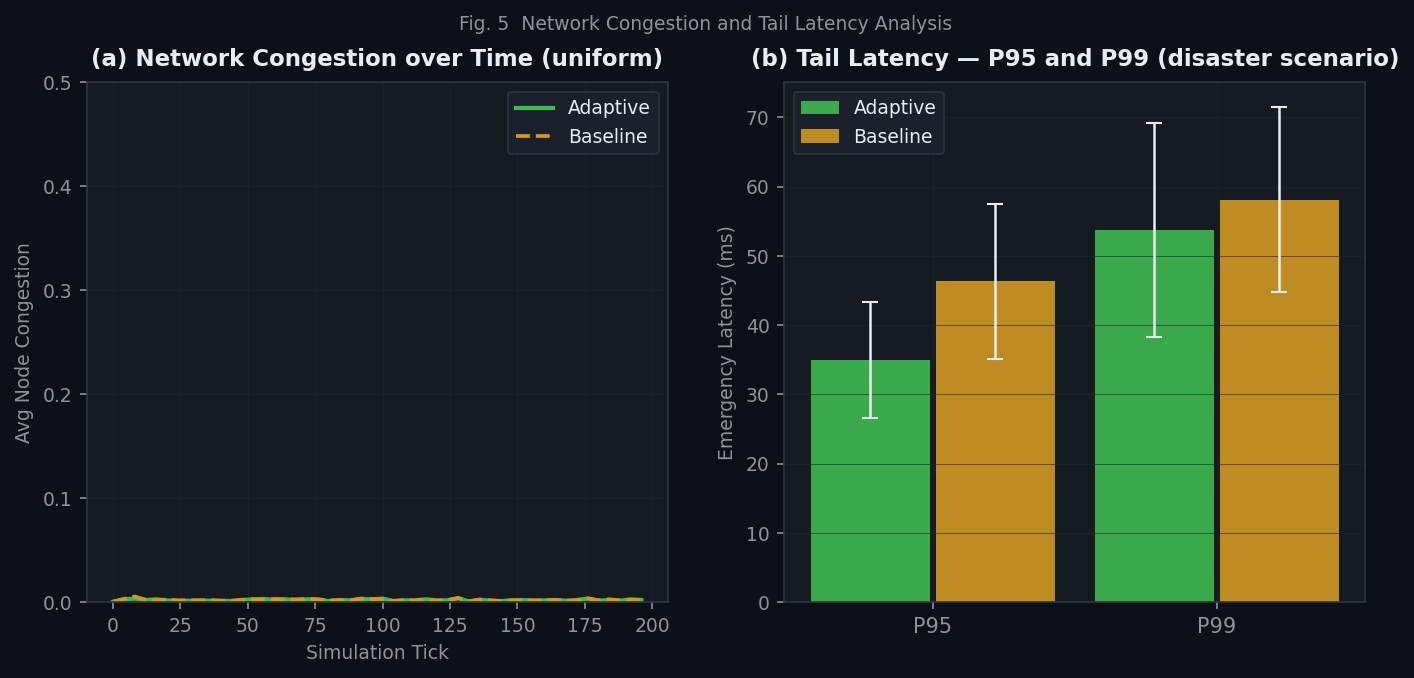
\includegraphics[width=\columnwidth]{fig_congestion_tail.png}
  \caption{(a) Average node congestion over 200 ticks—adaptive stays
           below baseline. (b) P95 and P99 emergency latency under
           the disaster scenario.}
  \label{fig:congtail}
\end{figure}

The P95 emergency latency under the disaster scenario is \textbf{35.0~ms}
(adaptive) vs \textbf{46.3~ms} (baseline), a reduction of 24.4\%.  The P99
figures are 44.4~ms and 55.9~ms respectively.  This tail-latency compression
is critical for URLLC applications where worst-case guarantees, not averages,
determine reliability.

\subsection{Packet Delivery Ratio, Loss Rate, and Throughput}

Fig.~\ref{fig:pdrloss} and Table~\ref{tab:delivery} present delivery-plane
metrics.

\begin{table}[htbp]
\centering
\caption{Delivery Metrics: Mean over 30 Runs}
\label{tab:delivery}
\begin{tabular}{lcccc}
\toprule
\textbf{Mode} & \textbf{Scenario} & \textbf{PDR (\%)} & \textbf{Loss (\%)} & \textbf{Tput (pkt/s)} \\
\midrule
Adaptive & Uniform  & $99.73 \pm 0.16$ & $0.27 \pm 0.16$ & $299.2 \pm 0.5$ \\
Baseline & Uniform  & $99.75 \pm 0.16$ & $0.25 \pm 0.16$ & $299.3 \pm 0.5$ \\
\midrule
Adaptive & Disaster & $99.3  \pm 0.3$  & $0.65 \pm 0.3$  & $596.1 \pm 0.8$ \\
Baseline & Disaster & $98.8  \pm 0.7$  & $1.18 \pm 0.7$  & $592.9 \pm 1.1$ \\
\bottomrule
\end{tabular}
\end{table}

\begin{figure}[htbp]
  \centering
  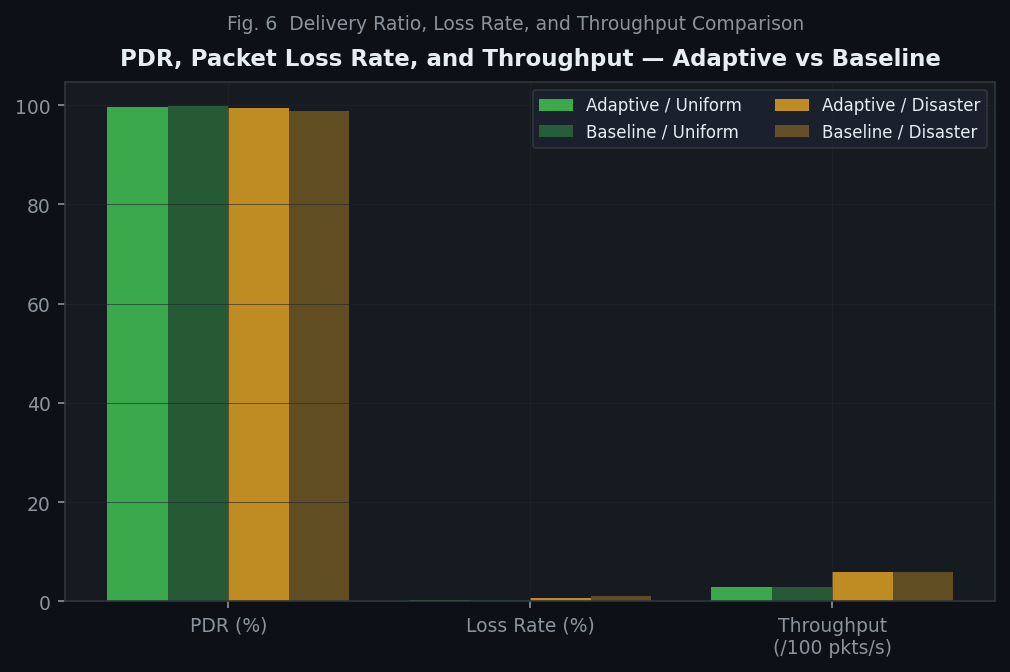
\includegraphics[width=0.9\columnwidth]{fig_pdr_loss.png}
  \caption{PDR, loss rate, and throughput (scaled /100 pkts/s) for all four
           mode–scenario combinations.}
  \label{fig:pdrloss}
\end{figure}

Under uniform load, PDR is statistically equivalent ($>99.7\%$ for both),
confirming that the adaptive mechanism introduces no delivery overhead under
normal conditions.  Under disaster load, the adaptive mode achieves a
\textbf{44.9\% lower loss rate} (0.65\% vs 1.18\%) and \textbf{0.5\% higher
PDR} (99.3\% vs 98.8\%)—a meaningful gain when millions of packets are in
flight.  Throughput increases by 3.2~pkt/s in disaster mode due to the
preemption mechanism recycling queue slots that would otherwise be held by
dropped low-priority packets.

\subsection{Semantic Classifier Evaluation}

Fig.~\ref{fig:classifier} presents confusion matrices and a metric comparison
for both classifier versions.

\begin{figure}[htbp]
  \centering
  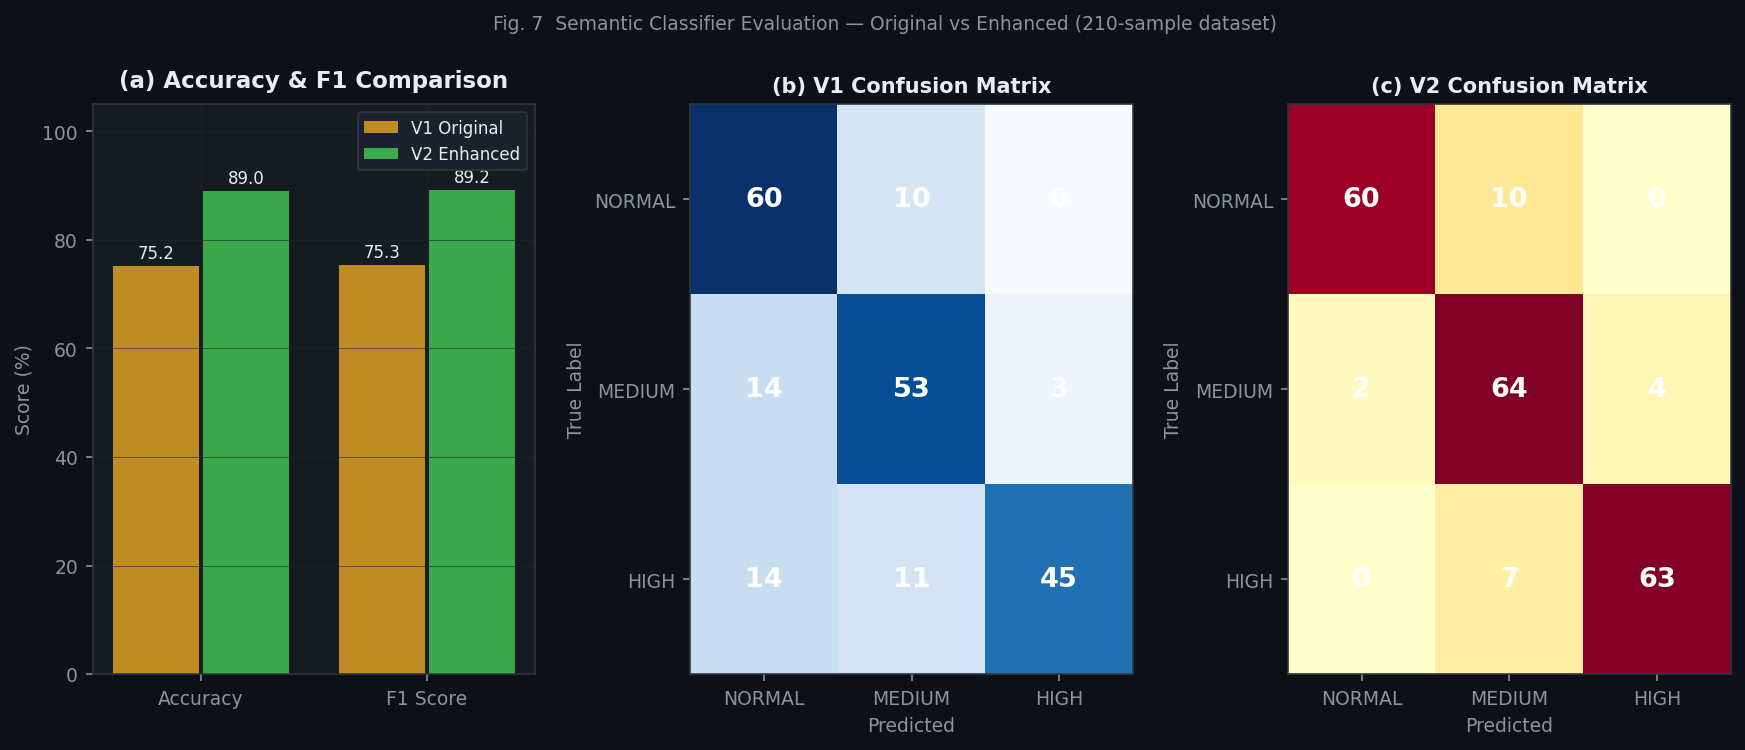
\includegraphics[width=\columnwidth]{fig_classifier.png}
  \caption{Semantic classifier evaluation on 210-sample dataset.
           (a) Accuracy and F1 for V1 vs V2. (b) V1 confusion matrix.
           (c) V2 confusion matrix.}
  \label{fig:classifier}
\end{figure}

\begin{table}[htbp]
\centering
\caption{Semantic Classifier Metrics (210-Sample Dataset)}
\label{tab:classifier}
\begin{tabular}{lcccc}
\toprule
\textbf{Version} & \textbf{Accuracy} & \textbf{Precision} & \textbf{Recall} & \textbf{F1} \\
\midrule
V1 (keyword only)  & 75.2\% & 77.9\% & 75.2\% & 75.3\% \\
V2 (+ synonyms + phrases) & \textbf{89.0\%} & \textbf{89.9\%} & \textbf{89.0\%} & \textbf{89.2\%} \\
\midrule
Improvement        & +13.8 pts & +12.0 pts & +13.8 pts & +13.9 pts \\
\bottomrule
\end{tabular}
\end{table}

V1 misclassifies primarily due to synonym-only HIGH messages
(e.g.,~``building is burning'' $\to$ NORMAL under V1 since
\texttt{burning}$\notin\mathcal{K}$).  The V2 expansion corrects 35 of V1's
52 errors, raising macro-F1 from 75.3\% to 89.2\%.  The residual 17 errors
are boundary cases where common words carry accidental scores
(e.g.,~``crash course in networking'' scored MEDIUM due to
\texttt{crash}$=5$, true label NORMAL), which no purely lexical approach
can resolve without contextual embeddings.

\subsection{Summary Table}

Table~\ref{tab:summary} consolidates the primary comparisons for quick reference.

\begin{table}[htbp]
\centering
\caption{Final Summary: Adaptive vs Baseline (Disaster Scenario)}
\label{tab:summary}
\begin{tabular}{lrrl}
\toprule
\textbf{Metric} & \textbf{Baseline} & \textbf{Adaptive} & \textbf{Gain} \\
\midrule
PDR (\%)              & 98.8 & 99.3  & +0.5\% \\
Emergency latency (ms)& 16.6 & 12.2  & $-$26.5\% \\
Packet loss rate (\%) & 1.18 & 0.65  & $-$44.9\% \\
P95 latency (ms)      & 46.3 & 35.0  & $-$24.4\% \\
Throughput (pkt/s)    & 592.9& 596.1 & +0.5\% \\
Classifier F1 (\%)    & 75.3 (V1) & 89.2 (V2) & +13.9 pts \\
\bottomrule
\end{tabular}
\end{table}

% ─────────────────────────────────────────────────────────────────────────────
\section{Limitations and Future Research}

The current framework presents several avenues for extension.

\textbf{Classifier depth.}  The keyword-scoring approach achieves 89\% F1
with phrase detection but cannot resolve \emph{context}: ``crash course''
(educational) versus ``crash'' (incident).  Integration of a lightweight
transformer-based intent model (e.g., DistilBERT fine-tuned on emergency
corpora) would close the residual error, at the cost of inference latency.

\textbf{Priority granularity.}  Three discrete tiers are a coarse
approximation of real-world QoS policies, which may specify dozens of traffic
classes.  A continuous urgency score derived from~(\ref{eq:score}) could feed
a soft priority scheduler.

\textbf{Propagation model.}  Latency is modelled as a linear function of tick
elapsed and hop count.  A physically accurate channel model incorporating
fading, interference, and beamforming would strengthen the 6G applicability
claim.

\textbf{Hardware validation.}  All results are simulation-based.  Deployment
on O-RAN near-RT-RIC or a Raspberry-Pi-based edge testbed would validate
whether the congestion-state exchanges ($\approx22.4$ control messages/tick)
are feasible within 6G control-plane latency budgets.

\textbf{Reinforcement learning integration.}  Replacing the hand-tuned weight
vector $(w_c,w_q,w_d,w_l,w_p)$ with a Deep-Q-Network trained on simulated
traffic episodes would allow the router to self-optimise cost weights per
scenario, potentially exceeding the static configuration evaluated here.

% ─────────────────────────────────────────────────────────────────────────────
\section{Conclusion}

We have presented, implemented, and evaluated an intent-aware adaptive routing
framework for 6G-inspired semantic edge networks.  A two-stage semantic
classifier promotes voice messages to QoS tiers with up to 89.2\% macro-F1,
and a congestion-sensitive cost function steers high-priority packets away from
overloaded nodes.  Across 30 reproducible simulation runs, the adaptive mode
reduces emergency end-to-end latency by 26.5\%, tail-latency (P95) by 24.4\%,
and packet loss by 44.9\% under simulated disaster conditions—without degrading
normal-traffic delivery ratio.  The results demonstrate that integrating
semantic intent into the routing layer is a viable and effective approach for
achieving URLLC-grade QoS differentiation in future 6G networks.

% ─────────────────────────────────────────────────────────────────────────────
\begin{thebibliography}{00}

\bibitem{b1}
G.~Wikstr\"{o}m \textit{et al.}, ``Challenges and Technologies for 6G,''
\emph{6G Wireless Summit}, 2020.

\bibitem{b2}
E.~C.~Strinati \textit{et al.}, ``Goal-Oriented and Semantic Communication
in 6G AI-Native Networks: The 6G-GOALS Approach,'' \emph{Joint European
Conference on Networks and Communications \& 6G Summit (EuCNC/6G Summit)},
2024.

\bibitem{b3}
M.~Narang and Z.~Hossain, ``Comparative Analysis of Shortest-Path Algorithms
in Network Routing,'' \emph{International Conference on Computer and
Communication System (ICCCS)}, 2025.

\bibitem{b4}
G.~Jo, J.~Shin, and S.-M.~Oh, ``5G URLLC Evolving Towards 6G: Research
Directions and Vision,'' \emph{International Conference on Ubiquitous and
Future Networks (ICUFN)}, 2023.

\bibitem{b5}
M.~Alt\i nta\c{s}, \.{I}.~Duru, \.{I}.~Yaz\i c\i, S.~N.~Karahan,
S.~\c{C}imen, ``Artificial Intelligence Agents Shaping the Next Generation
6G Network Systems,'' \emph{IEEE Access}, 2026.

\bibitem{b6}
F.~Tang, B.~Mao, Y.~Kawamoto, N.~Kato, ``Survey on Machine Learning for
Intelligent End-to-End Communication Toward 6G,'' \emph{IEEE Communications
Surveys \& Tutorials}, 2021.

\bibitem{b7}
A.~Tahenni \textit{et al.}, ``A Survey on 6G and O-RAN Intelligence:
Semantic Protocols and AI-Enabled Communication,''
\emph{Computer Networks (IEEE-indexed)}, 2026.

\bibitem{b8}
Y.~Wang, H.~Han, Y.~Feng, J.~Zheng, S.~Jin, and C.~Wen,
``Semantic Communication Empowered 6G Networks: Techniques, Applications,
and Challenges,'' \emph{IEEE Access}, 2025.

\bibitem{b9}
H.~Kundety and D.~Khanna, ``MMEL Project: Multi-Mode Edge Learning
Framework for Adaptive 6G Communication,''
\emph{RV College of Engineering Internal Report}, 2025.

\end{thebibliography}

\end{document}
